\documentclass[a4paper]{usiinfbachelorproject}

\captionsetup{labelfont={bf}}
%%%%%%%%%%%%%%%%%%%%%%%%%%%% PACKAGES %%%%%%%%%%%%%%%%%%%%%%%%%%%%%
\usepackage{float}
\usepackage{amsmath}

%%% Main Body %%%

\author{Costanza Rodriguez Gavazzi}

\title{\textbf{How do children search?}}
\subtitle{A tool to support researchers in understanding how children search for information online}
\versiondate{\today}

\begin{committee}

\advisor[Universit\`a della Svizzera Italiana, Switzerland]{ }{Monica }{Landoni }

\coadvisor[Universit\`a della Svizzera Italiana, Switzerland]{ }{Diletta Micol}{Tobia}

\end{committee}

\abstract {

As children increasingly engage in web searching activities both at home and in educational settings, understanding how they search for information has become a key topic in both Information Retrieval (IR) and Human-Computer Interaction (HCI). However, most search interfaces are designed for adults and fail to address the cognitive and emotional needs of younger users.
This thesis presents an interactive, web-based game designed to investigate how children search for information using either a traditional search engine or a Large Language Model (LLM). The game aims to be both engaging for children and practical for researchers. It logs structured interaction data, such as queries, tool preferences, session length, and user responses, and offers easy export of session logs for later analysis.

The project builds upon a previous prototype, making the system more modular, reusable, and suitable for real-world studies. Initial feedback from education professionals suggests the tool is promising as a research instrument, but still has room for improvement with respect to the user interface. This work provides a foundation for future iterations of the tool and supports the research community’s need for structured, quantitative data on children’s online information-seeking behavior.

\vspace{0.5em}

\textbf{Keywords}: Information Retrieval; Human-Computer Interaction; User Interface; Search Engine; LLM; Children;
}

\begin{document}
\maketitle
\tableofcontents
%\listoffigures\newpage

\newpage
%%%%%%%%%%%%%%%%%%%%%%%%%%%% INTRODUCTION %%%%%%%%%%%%%%%%%%%%%%%%%%%%%
\section{\textbf{Introduction}}

In recent years, children's interactions with search technologies have attracted growing attention in both Information Retrieval (IR) and Human-Computer Interaction (HCI). As the Internet becomes more common in schools and homes, children are learning to search for information on their own. However, their needs and behaviors are different from those of adults. Commercial search engines like Google and Bing are not built with children in mind, and they often overlook key aspects of children's cognitive and emotional development.

At the same time, large language models (LLMs) like ChatGPT\footnote{\url{https://openai.com/chatgpt}} and Gemini\footnote{\url{https://gemini.google.com}} have become increasingly popular among everyday users. While these models were not originally designed to replace search engines, many people now use them to look up information they would otherwise search for online. The single, focused response offered by an LLM is often seen as more convenient than going through a list of search results. Because of this, LLMs and search engines are now often viewed as interchangeable, even though they work very differently. These tools are also quickly evolving. Many models are now being developed with web browsing capabilities, allowing them to access real-time information. These systems combine LLMs with live web access to provide up-to-date answers, further closing the gap between conversational assistants and traditional search engines.

Previous research has shown that children struggle to evaluate search results effectively, particularly when results are presented in dense or complex formats. Moreover, their perception of what is relevant often differs from adult expectations and may be influenced by emotion, position in the list, or visual elements~\cite{Landoni2021c,Landoni2021b}.

This project builds on Savoia's 2025 thesis~\cite{Savoia2025}, which proposed a game to observe children's search behavior using both a traditional search engine and a chatbot-like Large Language Model (LLM) interface. Because the original prototype was a proof of concept, it did not implement a data collection feature. This thesis rebuilds that tool with the goal of creating a functioning and reusable prototype that can be used in real research scenarios and contribute to the development of child-friendly search tools.

To do this, the tool was designed as an interactive web-based game in which children answer questions framed in a neutral, positive, or negative emotional tone by choosing between two search tools. Their choices, search behavior, and answers are logged to generate structured data for research purposes. This allows to later analyze aspects such as tool preference, emotional influences, and performance across tasks.

This report is structured as follows:
\begin{itemize}
    \item Section 2 reviews background research and related work, providing motivation for the project.
    \item Section 3 explains how the requirements were defined and lists them.
    \item Section 4 describes the technical architecture of the system.
    \item Section 5 shows typical usage scenarios.
    \item Section 6 concludes the report with a discussion on the directions for future work.
\end{itemize}

%%%%%%%%%%%%%%%%%%%% BACKGROUND AND RELATED WORK %%%%%%%%%%%%%%%%%%%%%
\section{\textbf{Background and Related Work}}

The study of how children search for information online is a growing area that connects education, Information Retrieval (IR), and Human-Computer Interaction (HCI). The goal of this project was to develop a research tool that could collect interaction data from children using both traditional Search Engines and their Results Page (SERP), and Large Language Models (LLMs). Unlike other projects focused mainly on improving User Experience (UX) or User Interface (UI), this project was designed as a flexible platform to support various research questions on children's search behaviors. At the same time, the tool had to be fully functional and ready to use in real research scenarios, so an engaging and appropriate UI for younger users was still a key requirement.

\subsection{Foundation}

The starting point for this project was the bachelor's thesis by Savoia \cite{Savoia2025}. In her work, she proposed an interactive game designed to observe how children search for information. The interface was structured around a group of six islands, where each island represented a question framed with a specific emotional tone (positive, neutral, or negative). The children were allowed to choose how they wanted to answer the question, using a familiar web search interface or a chatbot-style LLM. Her work demonstrated that this narrative approach could encourage natural interactions and meaningful behavior from children.

Although her prototype successfully demonstrated the idea, it was not built with the core feature of data extrapolation, nor with reuse or extensibility in mind, but as a proof of concept. This project rebuilt the system from scratch to make it modular, maintainable, and suitable for future research experiments. Still, it kept the core idea of gameplay, the use of emotionally charged questions, and flexibility in tool choice to support various search strategies.

\subsection{Motivation}

A review of the literature highlighted the need for a research tool tailored to children's needs. Children are frequent users of Search Engines, especially in school settings, but often struggle to find relevant information efficiently \cite{Aliannejadi2021}. Most commercial tools like Google or Bing are designed for adults \cite{Aliannejadi2021, Landoni2021}, and there is no single search interface that fits all users, especially young people with different cognitive and emotional needs \cite{Landoni2021}.

In the IR research community, there is a clear call for child-friendly systems that are more suitable in educational contexts \cite{Landoni2020}. However, building such systems is challenging. Designing for children means taking into account their specific abilities: cognitive, technical, and emotional \cite{Chen2022}. In many cases, children say they want one thing, but their actual behavior shows something else. This is why relying only on interviews or post-task questionnaires can be misleading \cite{Aliannejadi2021}.

Besides, children are often left out of mainstream IR research and there is a lack of reliable data on how they really use search tools \cite{Savoia2025}. Researchers have highlighted the need for dedicated datasets, experimental tools, and evaluation methods designed for children \cite{Landoni2021c}.

Observing how children search and interact with systems, we can gather important insights that help improve the design of future tools \cite{Savoia2025}. These insights can also guide the development of features that help children, for example, by offering visual cues to highlight relevance or reduce confusion \cite{Landoni2021}. Data from child search behavior can also support many different research directions, including how emotions impact search performance, how children respond to positive or negative task formulation, or how task complexity affects engagement \cite{Landoni2020, Landoni2021c}. In particular, it is also interesting to consider how negative emotions are handled. Some research suggests that tracking negative user emotions could support better filtering, while others warn that hiding negative content could limit learning opportunities \cite{Landoni2020}.

A game-based tool, like the one built in this project, can collect structured data such as query logs, number of queries, time spent, and user clicks \cite{Aliannejadi2021}. It can also capture richer information on how children switch between tools or how many queries they need before answering. This kind of data would be difficult to gather with traditional observational methods or surveys, as children are reported to be unreliable sources when it comes to describing their own search behavior and preferences \cite{Aliannejadi2021}.

The strength of this approach comes from the benefits of game-based learning, which helps keep children engaged and motivated \cite{Alotaibi2024}. When children play a game, they tend to act more naturally and stay focused, making it easier to collect useful data on their behavior \cite{Alotaibi2024}. Compared to traditional learning environments, which can feel serious or stressful, games create a more relaxed space where children feel free to explore \cite{Alotaibi2024}.

By designing the tool as a digital game, we also benefit from interactive elements, storytelling, and visuals that make the experience fun.



\newpage

%%%%%%%%%%%%%%%%%%%%%%%%%%%% REQUIREMENTS %%%%%%%%%%%%%%%%%%%%%%%%%%%%%
\section{\textbf{Requirements}}

This project did not begin with a fixed list of specifications. Instead, requirements emerged iteratively through exploration of the research domain, analysis of related literature, and discussions with advisors, both researchers in IR and therefore stakeholders in this design space. The work builds on Savoia's thesis \cite{Savoia2025}, which included an initial prototype of the game that was tested in a pilot session with children. From that experience, the feedback from the advisors and what we found in the literature,a new version of the game came to life, one that is more functional, scalable, and better suited to support different research questions in IR and HCI, while also being engaging and usable for children.

The main objective was to implement a fully functional and reusable prototype that could collect detailed data on how children use traditional SE and LLM, while also being engaging and usable for children. The project extends Savoia's prototype \cite{Savoia2025}, which demonstrated the potential of a game-based framework to study children's search behavior, but did not actually integrate the aspect of user data collection.
To structure the design, this dual purpose of the tool was fundamental: relevance for researchers aiming to study search behavior, and a pleasurable and engaging experience for children. From this core duality, the following questions guided the requirements definition process:
To structure the design, the following questions guided the requirement definition process.
\begin{itemize}
    \item What kind of data do researchers want to collect?
    \item Can a game-based interface be used to collect these data effectively?
    \item What kind of game design is both engaging and suitable for structured data collection?
    \item How can the tool be both usable for researchers and appealing to children?
    \item How can the system be modular, extensible, and maintainable for future research?
    \item How can it adapt to different experimental setups or research contexts?
\end{itemize}

These reflections acted as a guide to explore the literature, which then led to a concrete list of functional and non-functional requirements, discussed below.

\subsection{Data for Research Use}
Research has shown that a variety of data is needed to understand children's search behaviors.
This includes both quantitative metrics and qualitative observations. Although qualitative observations can offer several advantages in designing for children, this project's main focus was on quantitative metrics to enable the identification of patterns or relationships among behaviors. Analysis of these patterns can help researchers identify the potential roles of searchers among children \cite{Imazu2017}. Understanding these distinct roles that children play when searching is a key element in characterizing their behavior. Previous research \cite{Foss2012} defined seven roles for children searching in a home setting, based on qualitative data such as interviews and observations. More recent research \cite{Landoni2021c} aimed to understand the search roles of children, specifically in the classroom, and to see if they could be inferred using a quantitative approach based on performance indicators from search logs and teacher evaluations. By analyzing quantitative data such as click accuracy, session length, and grades, researchers were able to identify patterns that corresponded to several of the original roles \cite{Landoni2021c}. These findings highlight that both qualitative and quantitative data are fundamental to understanding children's search behavior.


To do this, we identified the following types of data as relevant.

\begin{itemize}
    \item \textbf{Query Logs:} Query text, number of queries, and query term counts \cite{Aliannejadi2021, Savoia2025}.
    \item \textbf{Performance Indicators:} Session length, click counts, and rank depth \cite{Landoni2021c}.
    \item \textbf{Task Outcome Data:} Final user responses, with the idea that scoring based on teacher rubrics or predefined relevance criteria could be done later when analyzing the gathered data \cite{Landoni2021c}.
    \item \textbf{Tool Preference:} Children's selection patterns between search engine and LLM \cite{Savoia2025}.
    \item \textbf{Timing Data:} Time spent on each question, delays before interaction, and time spent on web pages \cite{Savoia2025}.
\end{itemize}


\subsection{UI Insights from Literature}

Designing a UI involves understanding how users interact with a digital system through visual and interactive elements. In this project, the UI was not the sole focus but because the target users were children, it required some careful thought. Designing UI for children presents challenges: it must be intuitive, engaging, and customized to their cognitive and emotional development. At the same time, the interface should allow adult stakeholders, such as teachers and researchers, to take any necessary actions, such as setting up the game and downloading the gathered data.

Considering the dual purpose of the tool, the following insights from the literature informed the UI design:

\begin{itemize}
    \item There is no one-size-fits-all SERP interface suitable for children \cite{Landoni2021}.
    \item Children prefer playful and engaging tools, and emotional design improves product recognition and user satisfaction \cite{Chen2022, Amin2022}.
    \item Humanized design elements such as avatars, animations, and storytelling are particularly effective for younger users \cite{Amin2022, Chen2022}.
    \item Participatory design methods show that children prefer familiar, usable UI elements but appreciate fun, cartoonish visuals \cite{Tapola2022, Landoni2021b}.
    \item Children prefer to interact with a tool they perceive to be similar to the real thing, instead of a simplified version \cite{Aliannejadi2021}.
    \item Based on their age and cognitive abilities, children require different levels of scaffolding \footnote{Scaffolding refers to a form of support provided in design, particularly for children \cite{Chen2022, Landoni2021c}. In app design, providing scaffolding involves conveying the goals of the app to children in an understandable way (i.e. interactive prompts, visual cues) \cite{Chen2022, Landoni2021c}} and support in search tasks \cite{Chen2022, Tapola2022, Amin2022}. In particular:

          \begin{itemize}

              \item \textbf{Ages 6 to 8:} Interfaces should use simple, familiar words, and reward systems are effective in maintaining engagement. Bright colors are still encouraged \cite{Amin2022}.

              \item \textbf{Ages 9 to 12:} These users value autonomy and prefer interfaces that offer control rather than instructions. Feedback should be informative rather than directive. Colors can be more subdued, such as green, grey, and navy tones. They are generally more skilled at navigating websites and handling smaller UI elements \cite{Amin2022}.
              \item
          \end{itemize}

\end{itemize}

\subsection{Functional Requirements}
Based on the insights from the literature and discussions with the advisors, the following functional requirements were defined for the system:

\subsubsection*{\textbf{Language and Initialization}}
\begin{itemize}
    \item The language of the game should be modular and easily changeable to be able to test the game with children from different countries.
    \item A landing page must appear before the game starts to allow teachers or researchers to explain the rules.
    \item The game must be reset when a new language is selected.
\end{itemize}

\subsubsection*{\textbf{Session Management}}
\begin{itemize}
    \item Each session must be identified by a unique user code provided by the teacher.
    \item The game must start only after the user inputs a valid code.
    \item The game must persist its state on page refresh using local storage.
    \item Researchers must be able to download session data at any time, even if the game is incomplete.
    \item When downloading data, the system must request a password to protect the export and prevent children from tampering with it.
\end{itemize}

\subsubsection*{\textbf{Gameplay Logic}}
\begin{itemize}
    \item The game must include six clickable islands, presented in a randomized order per session.
    \item Islands can be clicked in any order.
    \item Each island represents a straightforward question with a specific emotional framing: positive, neutral, or negative.
    \item Once answered, an island becomes inactive and cannot be clicked again.
    \item Inactive islands must show a different cursor, remove hover effects, and a message should appear when trying to click on them.
    \item Each completed island increases the score by 10 points (maximum 60).
    \item The current score must be shown to motivate the user.
\end{itemize}

\subsubsection*{\textbf{Search Tool Interfaces}}
\begin{itemize}
    \item Clicking on an island must open a question page where the user chooses between two different search tools: Google or Gemini (LLM).
    \item Users must be allowed to switch between the two tools freely before submitting an answer.
    \item The Google interface must visually mimic a real search engine and display the top 10 results.
    \item The Gemini interface must mimic a realistic chatbot interface.
    \item Clicking on a Google result must open the link in a new browser tab.
\end{itemize}

\subsubsection*{\textbf{User Interaction Tracking}}

The system must record \textbf{per-island data}:

\begin{itemize}
    \item Question
    \item Sentiment of the question
    \item Time of the first click on the island
    \item Time of the answer submission for the island
    \item A list of objects containing information about each query or prompt performed by the user, in particular:
          \begin{itemize}
              \item If the query was made using Google or Gemini
              \item The text of the query or prompt
              \item The number of query terms
              \item The answer provided by the tool of choice - either a list of SERP results for Google or the response from Gemini.
              \item When saving SERP results, the system must record: \begin{itemize}
                        \item The title of the result
                        \item The snippet of the result
                        \item The position of the result in the SERP
                        \item The order in which the result was clicked
                        \item The time spent on the page corresponding to the result
                    \end{itemize}
          \end{itemize}
    \item The user's final submitted answer
\end{itemize}

The system must also record \textbf{per-session data}:
\begin{itemize}
    \item Language of the game
    \item A code to identify the session, provided by the teacher
    \item Start time and finish time of the session
    \item Session length
    \item The order in which the islands were completed
    \item The order in which the islands were clicked
    \item Total number of clicks in the session
    \item The time before the first click in the session
    \item The final score of the session
\end{itemize}


\subsubsection*{\textbf{User Experience and Engagement}}
\begin{itemize}
    \item The game must allow revisiting of islands before submission.
    \item The emotional tone must be visually represented with colors or icons.
    \item The User Interface must balance playful and realistic design to reflect real-world behavior of children when interacting with games.
    \item Upon completion, a thank you page must show the user's final score.
    \item The background includes animations to enhance engagement.
\end{itemize}

\newpage

%%%%%%%%%%%%%%%%%%%%%%%%%%%% SYSTEM DESIGN %%%%%%%%%%%%%%%%%%%%%%%%%%%%%
\section{\textbf{System Design}}

\subsection{Overview}

The game is implemented as a single-page web application developed using React, a JavaScript framework. The architecture follows a standard component-based design, where each part of the user interface is a block, potentially reusable. All logic, including game progression, timing, data collection, and API communication, is embedded directly in the relevant components or custom hooks.

There is no back-end: the entire game runs in the user's browser. State is managed using React's Context API and saved to \texttt{localStorage} to support persistence across sessions. When needed, the app communicates with external APIs to retrieve results from a search engine (Google) or a large language model (Gemini).


\subsection{Structure}

The main components of the application represent the major stages of the game and are shown in Fig.~\ref{fig:architecture}. The flow begins at \texttt{ChooseLanguagePage} and proceeds through \texttt{GameStartPage}, \texttt{MapPage}, \texttt{ChoicePage}, and \texttt{QuestionPage}, concluding at \texttt{FinishPage}.

While some transitions are one-way (e.g., from start to map), the design supports two-way navigation between \texttt{MapPage}, \texttt{ChoicePage}, and \texttt{QuestionPage}, allowing users to explore and revisit islands freely. The state and data collected during navigation are tracked using a centralized context. The \texttt{QuestionPage} triggers asynchronous calls to either the Google Search API or the GoogleGenerativeAI API, based on the user's choice.


\begin{center}
    \includegraphics[width=0.9\textwidth]{figures/architecture.png}
    \captionof{figure}{Structure of the application.}
    \label{fig:architecture}
\end{center}



\subsection{APIs}

The game uses two external services in order to retrieve the information from the user's prompts, selected based on the player's choice:

\begin{itemize}
    \item \textbf{Google Search API} \\
          Executes a custom Google search and retrieves the top 10 results for a given query. When users select the \textit{Google} option in \texttt{ChoicePage}, this API returns search engine results, each including metadata such as title, snippet, rank, whether it was clicked, click order, and time spent on the result.

    \item \textbf{GoogleGenerativeAI API (Gemini)} \\
          Sends the user's prompt to the Gemini LLM and returns a generated answer. This is selected when the player chooses the \textit{Gemini} option. Responses are stored in the local state alongside metadata such as prompt length and timestamp.
\end{itemize}


\subsection{Technologies Used}

The application is built using the \textit{Create React App} boilerplate, which provides a pre-configured setup for React applications. The main technologies used are:

\begin{itemize}
    \item \textbf{React}: Core framework for building the single-page application with reusable components and hooks.
    \item \textbf{JavaScript}: Used for writing all the game logic and component logic.
    \item \textbf{Mantine UI}: A React component library.
    \item \textbf{Plain CSS}: Used for styling components, organized in modular files like \texttt{map.css}, \texttt{question.css}, and more.
    \item \textbf{Google Custom Search API}: Used to perform keyword-based queries when users choose the “Google” source.
    \item \textbf{GoogleGenerativeAI API (Gemini)}: Provides LLM-based responses to user prompts when the “Gemini” option is selected.
    \item \textbf{React Context + Hooks}: For managing shared state (e.g., game data, API responses).
    \item \textbf{Browser LocalStorage}: Saves session data, including game state and interaction logs.
    \item \textbf{Environment Variables (.env)}: API keys are stored in a private .env file and accessed at runtime.
\end{itemize}

Custom utility hooks such as \texttt{useWindowDimensions} and \texttt{useAutoScale} dynamically adapt the UI layout. Global game state is managed with React's Context API in the \texttt{GameStateContext} component.


\subsection{Research Data Collection}

The game collects structured data to support research on how users interact with different information sources (search engine vs. large language model). All data is stored locally and can be exported at the end of the session.

\begin{itemize}
    \item \textbf{Session Metadata}:
          \begin{itemize}
              \item \texttt{userCode}, \texttt{startTime}, \texttt{finishTime}, \texttt{sessionLength\_seconds}
              \item \texttt{totalClicksInSession}, \texttt{islandClickOrder}, \texttt{islandCompletionOrder}
          \end{itemize}
    \item \textbf{Per-Island Data}:
          \begin{itemize}
              \item \texttt{question}, \texttt{sentiment}, \texttt{userAnswer}
              \item \texttt{choiceForAnswer}: Logs whether the user chose Google (0) or Gemini (1)
              \item \texttt{Queries}: Contains detailed records of each query:
                    \begin{itemize}
                        \item \texttt{query}: Text of the input, \texttt{AI}: Flag (0 for Google, 1 for Gemini), \texttt{numberOfQueryTerms}, \texttt{answer}: Either a plain string (for Gemini) or a list of search results (for Google), each entry made of title, snippet, position, click status, click order, time spent on result
                    \end{itemize}
          \end{itemize}
\end{itemize}

All of this information can be exported via the \texttt{exportData()} function and analyzed to study user behavior, preference trends, and differences between information retrieval strategies. An example of the exported data is shown in Appendix~\ref{app:exported-data}.

\newpage
%%%%%%%%%%%%%%%%%%%%%%%%%%%% USAGE SCENARIOS %%%%%%%%%%%%%%%%%%%%%%%%%%%%%

\section{\textbf{Usage Scenarios}}

This section illustrates how researchers or teachers (stakeholders) can set up the game and download the data, and how a child interacts with it during a typical session.

\subsubsection*{\textbf{Step 1: Language Selection}}

The game begins with the language choice screen (Fig.~\ref{fig:language-choice}). The stakeholders select their preferred language before continuing, setting up the game for the child. A hover effect provides visual feedback (Fig.~\ref{fig:language-hover}).

\begin{figure}[H]
    \begin{minipage}[b]{0.5\textwidth}
        \centering
        \includegraphics[width=0.9\textwidth]{figures/language-choice.png}
        \caption{Language choice screen.}
        \label{fig:language-choice}
    \end{minipage}%
    \hfill
    \begin{minipage}[b]{0.5\textwidth}
        \centering
        \includegraphics[width=0.9\textwidth]{figures/language-hover.png}
        \caption{Hover effect on language choice.}
        \label{fig:language-hover}
    \end{minipage}
\end{figure}

\subsubsection*{\textbf{Step 2: Session Start}}

After an adult has chosen the language, the child sees the start screen of the game (Fig.~\ref{fig:start-page}). A hover animation was implemented, guiding them to start (Fig.~\ref{fig:start-hover}).

\begin{figure}[H]
    \begin{minipage}[b]{0.5\textwidth}
        \centering
        \includegraphics[width=0.9\textwidth]{figures/start-page.png}
        \caption{Game start screen.}
        \label{fig:start-page}
    \end{minipage}%
    \hfill
    \begin{minipage}[b]{0.5\textwidth}
        \centering
        \includegraphics[width=0.9\textwidth]{figures/start-hover.png}
        \caption{Hover effect on start button.}
        \label{fig:start-hover}
    \end{minipage}
\end{figure}

\subsubsection*{\textbf{Step 3: Entering a Code}}

The system requires the child to enter the session code they received prior to the start of the session (Fig.~\ref{fig:code-check}), which is validated (Fig.~\ref{fig:code-ok}). This ensures that all recorded data is associated with a specific session.

\begin{figure}[H]
    \begin{minipage}[b]{0.5\textwidth}
        \centering
        \includegraphics[width=0.9\textwidth]{figures/code-check.png}
        \caption{Session code entry screen.}
        \label{fig:code-check}
    \end{minipage}%
    \hfill
    \begin{minipage}[b]{0.5\textwidth}
        \centering
        \includegraphics[width=0.9\textwidth]{figures/code-ok.png}
        \caption{Successful code validation.}
        \label{fig:code-ok}
    \end{minipage}
\end{figure}

\subsubsection*{\textbf{Step 4: The Island Map}}

The core component of the game corresponds to the map page (Fig.~\ref{fig:map}). Each of the six clickable islands represents a unique search task. The hover feedback (Fig.~\ref{fig:map-hover}) helps guide the attention of the children.


\begin{figure}[H]
    \begin{minipage}[b]{0.5\textwidth}
        \centering
        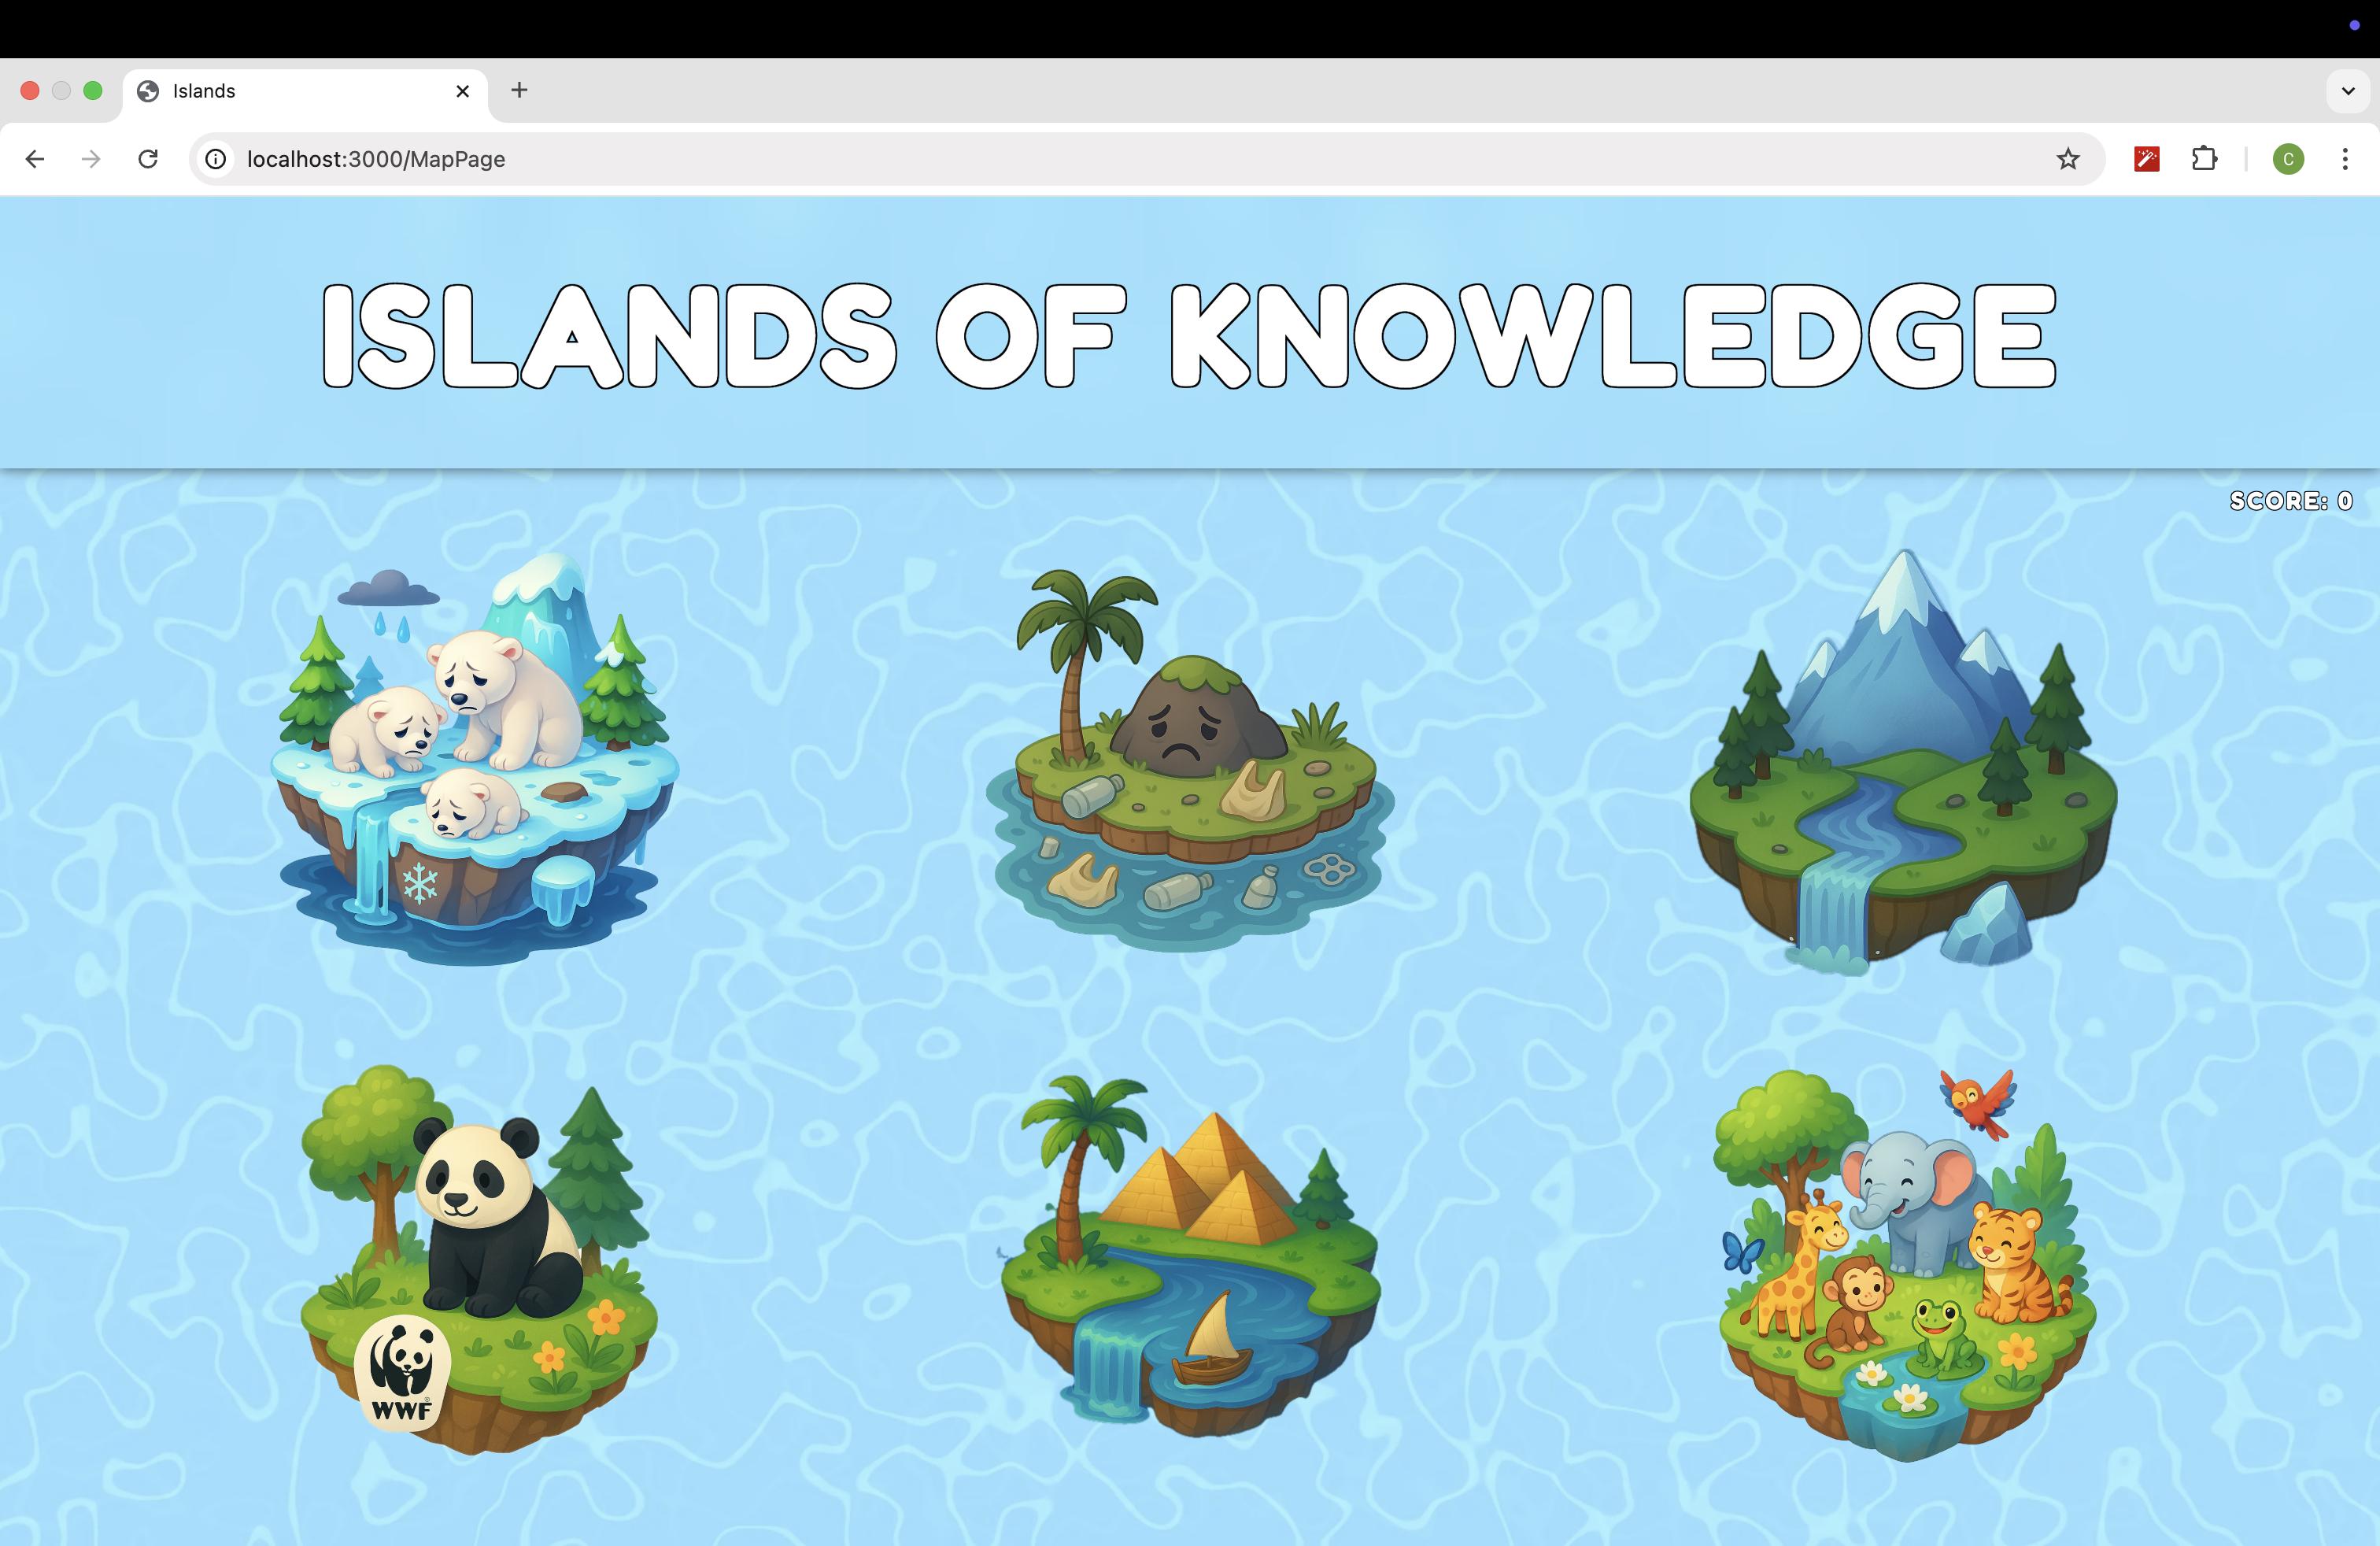
\includegraphics[width=0.9\textwidth]{figures/map.png}
        \caption{Island map with clickable islands.}
        \label{fig:map}
    \end{minipage}%
    \hfill
    \begin{minipage}[b]{0.5\textwidth}
        \centering
        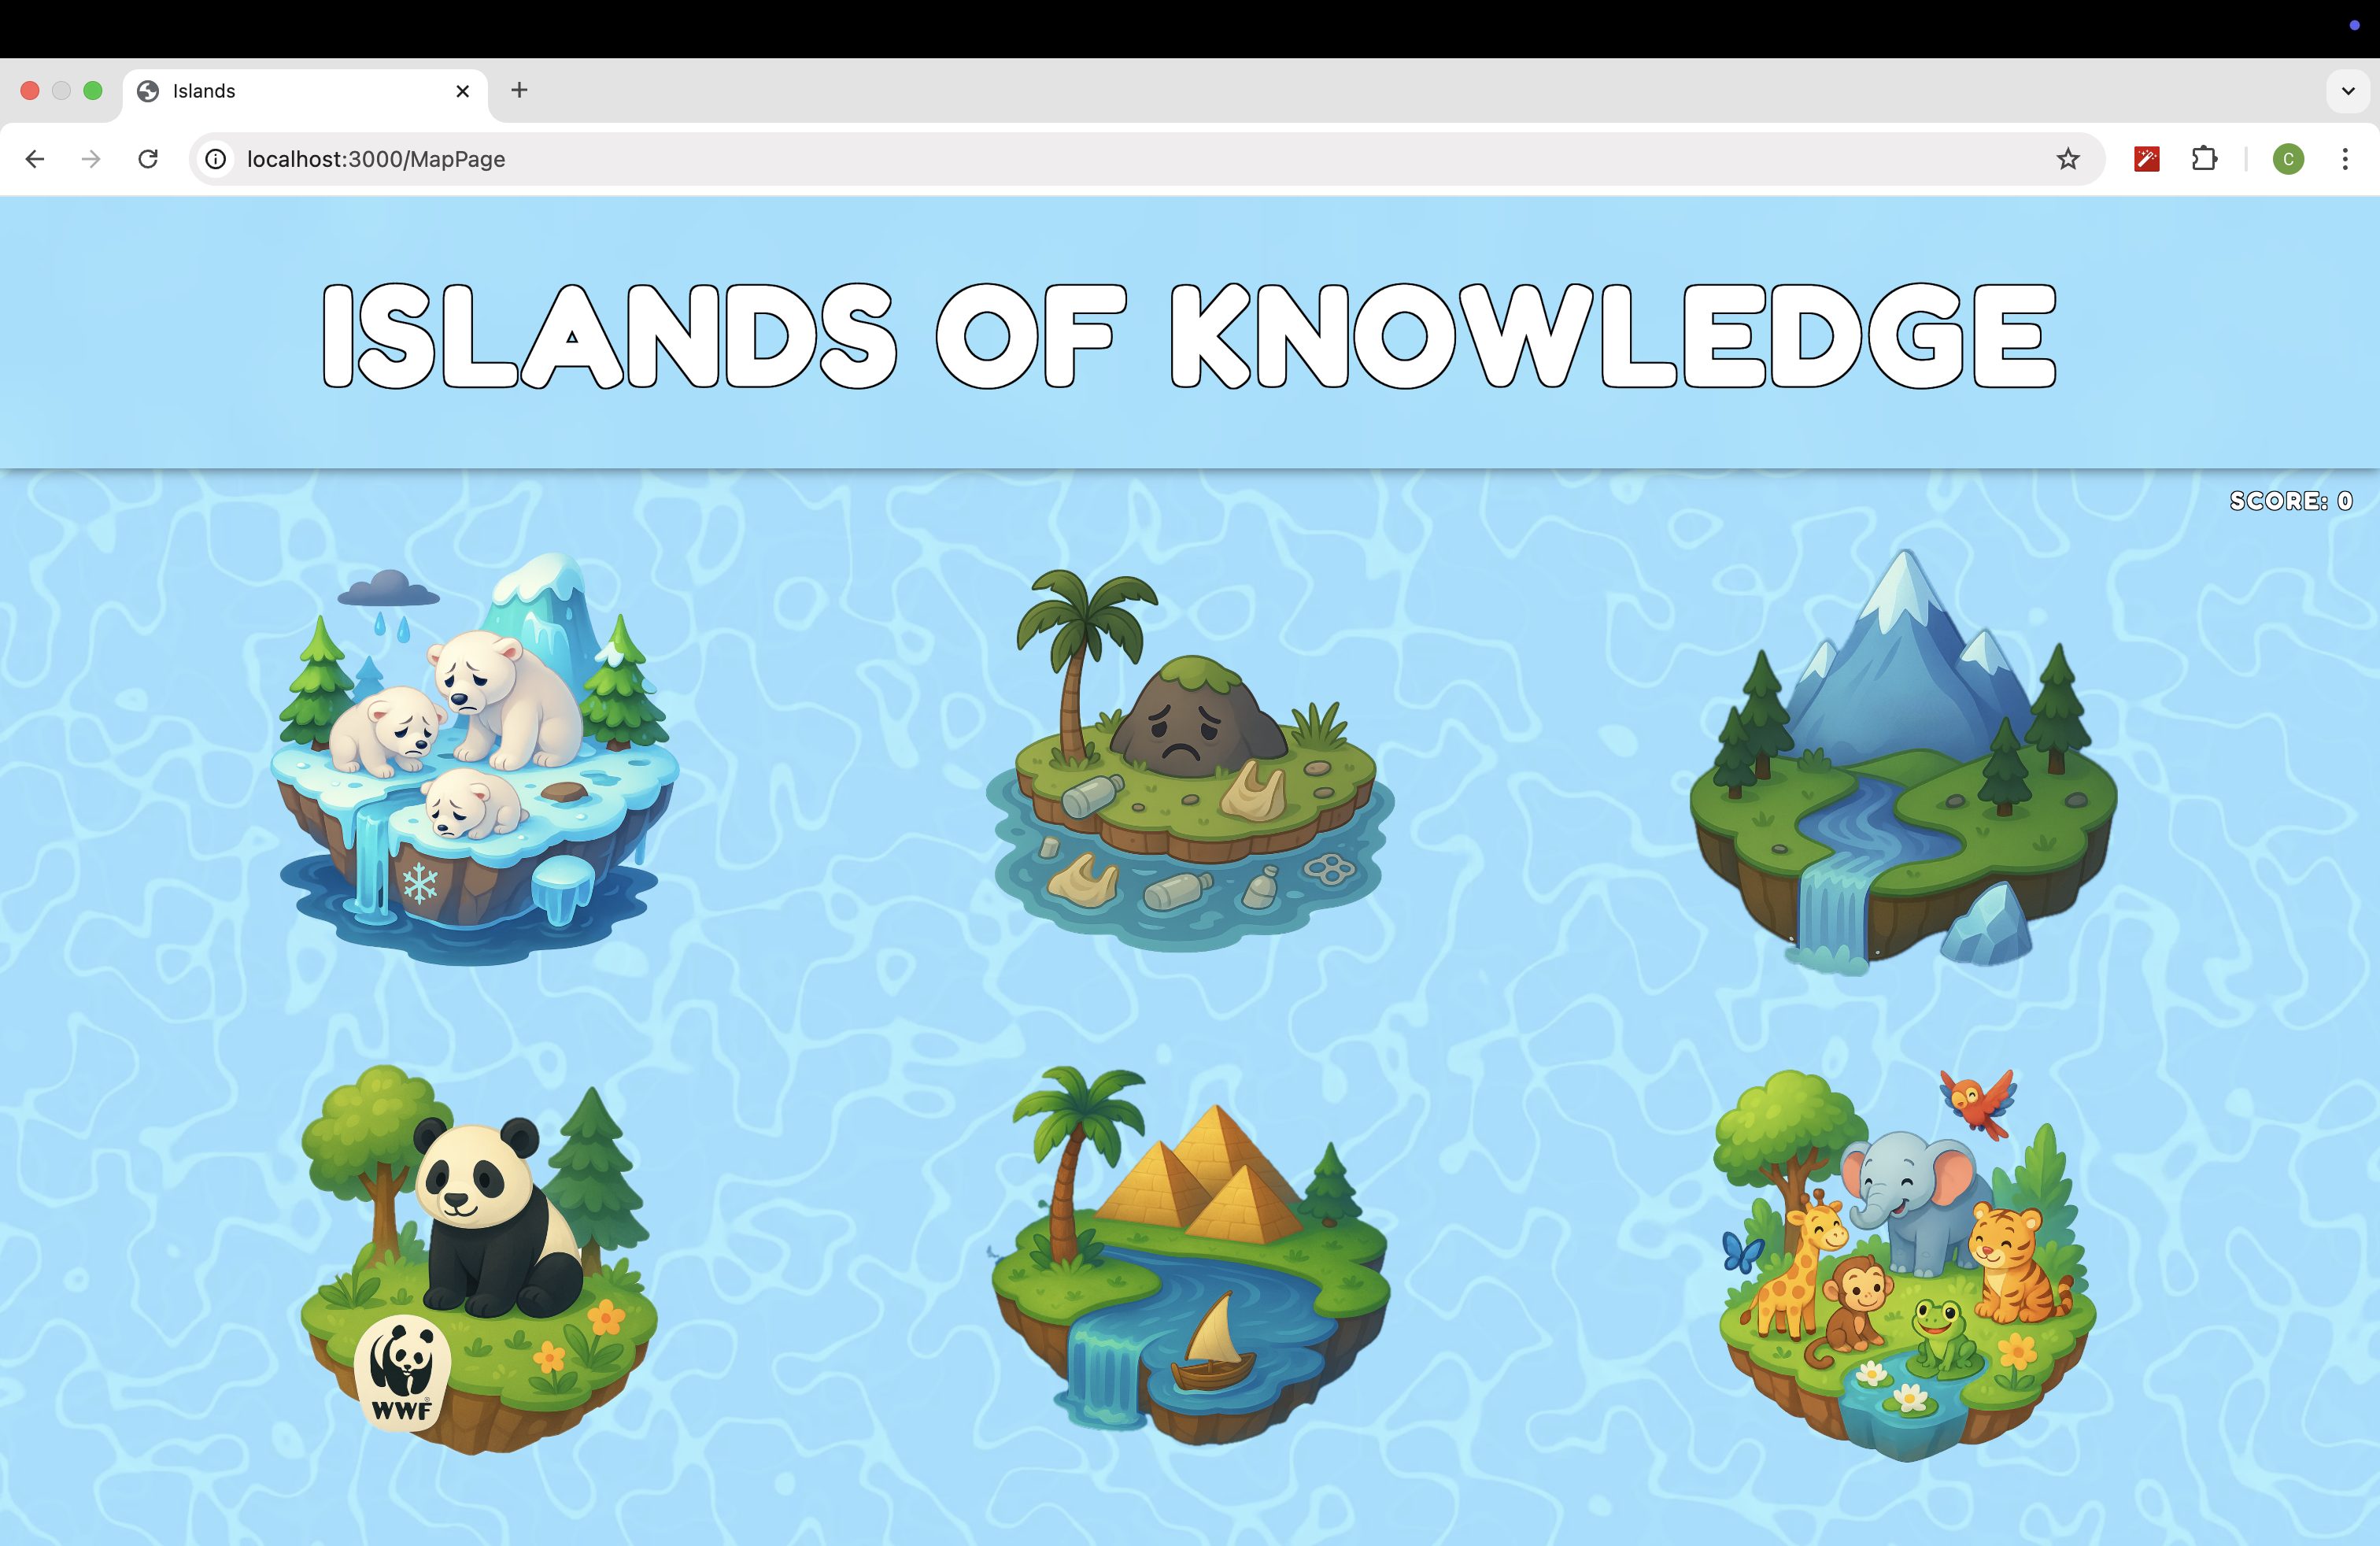
\includegraphics[width=0.9\textwidth]{figures/map-hover.png}
        \caption{Hover effect on islands.}
        \label{fig:map-hover}
    \end{minipage}
\end{figure}

\subsubsection*{\textbf{Step 5: Tool Choice}}

After selecting an island, the child reaches a tool selection page (Fig.~\ref{fig:choice-page}) where they choose between a traditional search engine (Google) and a large language model (Gemini).

\begin{figure}[H]
    \centering
    \includegraphics[width=0.5\textwidth]{figures/choice-page.png}
    \caption{Tool choice screen.}
    \label{fig:choice-page}
\end{figure}

\subsubsection*{\textbf{Step 6: Using Google}}

If the child selects Google, they are presented with a simulated Search Engine landing page (Fig.~\ref{fig:google}). The interface and behavior mimic real-life scenarios (Fig.~\ref{fig:serp}). Clicking on links opens them in a new tab.

\begin{figure}[H]
    \begin{minipage}[b]{0.5\textwidth}
        \centering
        \includegraphics[width=0.9\textwidth]{figures/google.png}
        \caption{Simulated Google landing.}
        \label{fig:google}
    \end{minipage}
    \hfill
    \begin{minipage}[b]{0.5\textwidth}
        \centering
        \includegraphics[width=0.9\textwidth]{figures/serp.png}
        \caption{Google search results with clickable links.}
        \label{fig:serp}
    \end{minipage}%
\end{figure}

\subsubsection*{\textbf{Step 7: Using Gemini}}

Alternatively, children can choose Gemini, where a chat-like interface appears (Fig.~\ref{fig:gemini}). A waiting screen mimics the LLM response delay after sending a prompt (Fig.~\ref{fig:gemini-waiting}), followed by the result output (Fig.~\ref{fig:gemini-results}).

\begin{figure}[H]
    \begin{minipage}[b]{0.5\textwidth}
        \centering
        \includegraphics[width=0.9\textwidth]{figures/gemini.png}
        \caption{Gemini chat interface.}
        \label{fig:gemini}
    \end{minipage}%
    \hfill
    \begin{minipage}[b]{0.5\textwidth}
        \centering
        \includegraphics[width=0.9\textwidth]{figures/gemini-waiting.png}
        \caption{Waiting screen for Gemini response.}
        \label{fig:gemini-waiting}
    \end{minipage}
    \begin{minipage}[b]{0.5\textwidth}
        \centering
        \includegraphics[width=0.9\textwidth]{figures/gemini-results.png}
        \caption{Gemini response output.}
        \label{fig:gemini-results}
    \end{minipage}
\end{figure}

\subsubsection*{\textbf{Step 8: Submitting an Answer}}

After exploring the results, the child can type the final answer (Fig.~\ref{fig:answer}). Once submitted, the user is redirected to the map page, and the island becomes inactive. If the child attempts to revisit a completed island, a warning is shown (Fig.~\ref{fig:warning}).

\begin{figure}[H]
    \begin{minipage}[b]{0.5\textwidth}
        \centering
        \includegraphics[width=0.9\textwidth]{figures/answer.png}
        \caption{Final answer submission screen.}
        \label{fig:answer}
    \end{minipage}%
    \hfill
    \begin{minipage}[b]{0.5\textwidth}
        \centering
        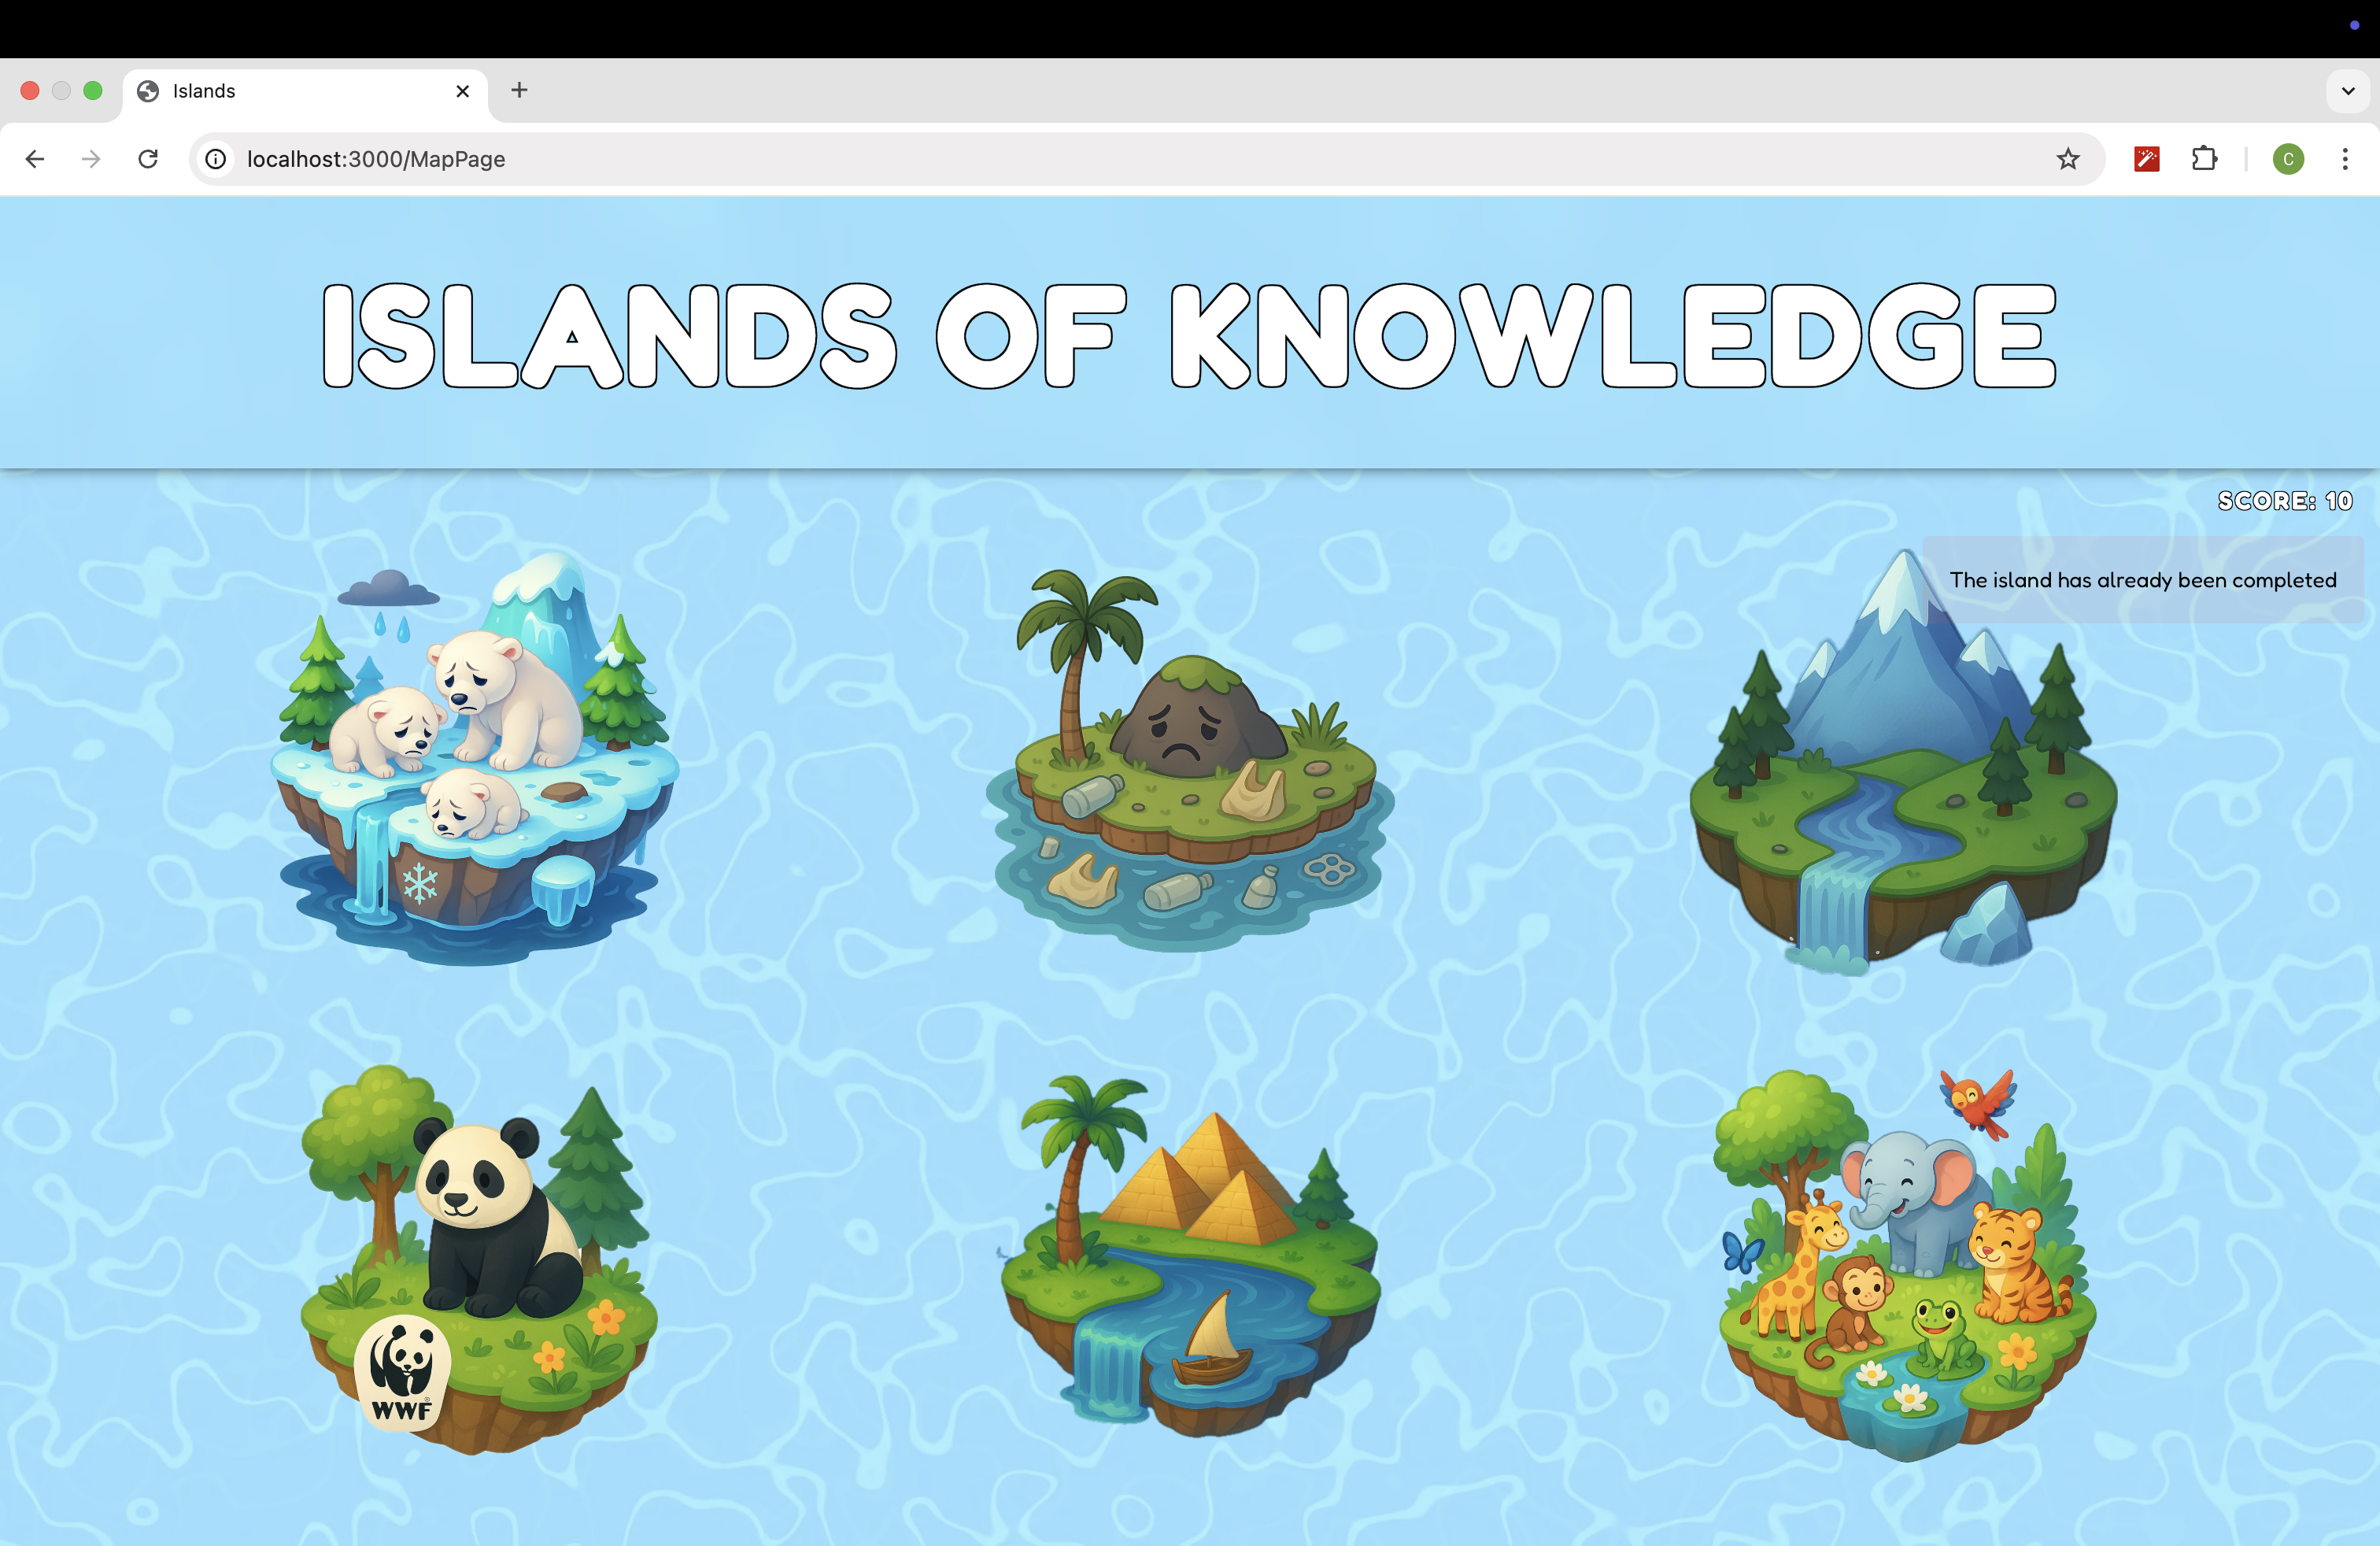
\includegraphics[width=0.9\textwidth]{figures/warning.png}
        \caption{Can't click on a completed island.}
        \label{fig:warning}
    \end{minipage}
\end{figure}

\subsubsection*{\textbf{Step 9: Final Page and Data Export}}

After completion of all six islands, the child sees their final score (Fig.~\ref{fig:final-score}). Each completed island contributes 10 points, with a maximum of 60.

To end the session, a password-protected download prompt is shown (Fig.~\ref{fig:download}), allowing the teacher or researcher to save all session data locally. It was a design choice to use the browser's prompt functionality instead of a custom modal, to discourage children from trying to tamper with the data export.

\begin{figure}[H]
    \begin{minipage}[b]{0.5\textwidth}
        \centering
        \includegraphics[width=0.9\textwidth]{figures/final-score.png}
        \caption{Final score screen after completing all islands.}
        \label{fig:final-score}
    \end{minipage}%
    \hfill
    \begin{minipage}[b]{0.5\textwidth}
        \centering
        \includegraphics[width=0.9\textwidth]{figures/download.png}
        \caption{Password-protected data download prompt.}
        \label{fig:download}
    \end{minipage}
\end{figure}

\subsection{\textbf{Experts' Feedback}}

The tool was presented to three teachers with experience working with children and technology. They provided valuable feedback on the design and usability of the tool, which should be discussed during future iterations of development. Please note that the feedback should be considered as input to be discussed and further analyzed, rather than as definitive requirements to be implemented.

\begin{enumerate}

    \item The overall visual design was considered slightly outdated and overly childlike, more appropriate for younger students (third or fourth grade). Both experts suggested a more modern and polished look to better suit the target age group.
    \item Regarding the first screen, the introductory message was described as too long. Since children tend to click instinctively, they might skip important instructions. To address this, two alternative solutions were proposed:
          \begin{enumerate}
              \item Split the prompt into two screens, one with a warning to wait for the teacher's instruction, and a second screen with a clickable button.
              \item Using a larger font and shortening the text (e.g., “\textit{WAIT! When you hear 'ok', click}”).
          \end{enumerate}

    \item The screen featuring clickable islands was deemed not intuitive. The experts noted that it did not encourage interaction and that some children might not realize that the elements were clickable. Additionally, the use of happy and sad face icons was discouraged, as they could lead children to assign emotional meaning or personify the interface unnecessarily.
    \item For the question screen, both font size and type were mentioned. They believed that the text should be larger and use a highly readable font such as Arial or certified dyslexia fonts. Furthermore, the question area was suggested to be visually highlighted (e.g., with a colored background) to make it stand out from the rest of the interface.
    \item The use of commercial logos was also criticized. This was flagged both for ethical reasons and for inconsistency: although a Google-like logo was shown, the following screen was considered not an accurate replica of the Google or Gemini interface. As a workaround, it was recommended to label the search interface simply as “\textit{Search Engine}” while mimicking the Google look through color and font style.
    \item The score system also received mixed feedback. It was suggested to give teachers the option to enable or disable the display of points. For children with lower self-esteem, visible scores could be discouraging. In contrast, group dynamics could benefit from visible scoring as a form of motivation. If scores are shown, they should be designed with engaging, attention-grabbing visuals.
    \item The simulated Google interface needed refinement. The space for displaying the question was perceived as difficult to notice, and the answer input field was not clearly interactive. Improving layout cues would help clarify the expected user action.
    \item The final screen's thank-you message was considered too long. A concise alternative such as “\textit{Great job! You earned X points!}” was recommended, particularly if the scoring feature remains active.
    \item One teacher raised a concern about the lack of scaffolding during the research phase of the game as younger students may require structured support to conduct meaningful searches. It was suggested to provide curated websites alongside guiding questions, ensuring students are able to find suitable information independently without being overwhelmed.
    \item AUDIO WHATSAPP TODO

\end{enumerate}



These insights are essential to improve both the usability and accessibility of the tool in future versions.


\newpage

%%%%%%%%%%%%%%%%%%%%%%%%%%%% CONCLUSIONS %%%%%%%%%%%%%%%%%%%%%%%%%%%%%

\section{\textbf{Conclusions}}

This project focused on the design and development of a tool to support researchers collecting user data to study how children interact with different information retrieval systems. The tool, designed in collaboration with researchers and teachers and built as an interactive web-based game, allows children to choose between a traditional search engine and a chatbot-style LLM to answer emotionally framed questions. All interactions are logged in a structured way, enabling the collection of data to support research.

The work originated from the limitations identified in Savoia's thesis \cite{Savoia2025}, particularly the need for data collection features. While her work laid the foundation for a possible approach to studying search behavior, it did not provide a usable or extensible tool for research purposes. This project rebuilt the system with the aforementioned goals in mind.

Several contributions were achieved:
\begin{itemize}
    \item A fully functional prototype was implemented.
    \item A data model was developed to log user interactions in detail, capturing a variety of metrics relevant to IR and HCI research.
    \item The user interface was designed to balance child-friendly visuals with realistic representations of search interfaces, aligning with guidelines from the literature.
    \item Feedback from experts in education and child-computer interaction was gathered to inform future improvements and highlight potential issues in usability.
\end{itemize}

The project provides a functional addition to current state of the art in the IR and HCI research domains, particularly in the context of studying children's search behavior. The tool is designed to be modular and extensible, allowing for future adaptations to different research contexts or experimental setups.

\subsection{\textbf{Future Work}}

Although the current prototype is functional and is already suitable for small-scale research studies, further improvements can be made in future iterations to improve usability, data collection, and scalability.

\subsubsection*{\textbf{User Interface and Usability Testing}}
The current interface was designed based on the insights of the literature and internal feedback, but because the design interface could have been a whole project on its own, it can be improved. Furthermore, it has not yet been tested with children in real-life settings. One key area for future work is to conduct formal usability testing sessions with children of different age groups. These sessions would help identify which parts of the UI are intuitive, which are appealing, and which are confusing or too complex. For example, visual feedback (for example hover animations, tool choices, iconography) may need to be adjusted based on children's preferences and cognitive abilities. Additionally, working with experts in child-computer interaction and UX/UI could help refine the design to better suit the target audience.

\subsubsection*{\textbf{Extending Data Collection}}

The current version of the system already collects a wide set of interaction data, including query logs, tool switches, time spent, and submitted responses. However, there is room for improvement and expansion. Future versions could include additional behavioral signals, such as
\begin{itemize}
    \item Mouse movement and hover times to infer hesitation or curiosity.
    \item Scroll depth within the SERP.
    \item Optional feedback prompts for children to self-report satisfaction or perceived difficulty.
\end{itemize}


\subsubsection*{\textbf{Improving Efficiency and Scalability}}

In the current version of the system, all interaction data is stored locally in the browser and must be manually exported at the end of each session. Although this solution is suitable for small-scale studies or pilot experiments, it introduces several limitations when conducting larger studies.

Managing data from multiple devices becomes time-consuming and there is a risk of losing session data if a participant closes the browser before exporting. Relying on browser-based password prompts also provides only minimal protection and may not be ideal in more formal research contexts.

A possible solution could be to integrate a back-end infrastructure that stores the data in a centralized manner, allowing researchers to:
\begin{itemize}
    \item Monitor sessions in real time, even across multiple classrooms or devices.
    \item Automatically collect and aggregate data without manual intervention.
    \item Minimize the risk of data loss due to user error or technical problems.
\end{itemize}

\subsubsection*{\textbf{Architecture and Code Quality}}
The current codebase is functional but there is always room for improvement. Future work could focus on separating the logic from the UI components, implementing a separate layer for game functionality, and using a more modular architecture. Ths refactoring would further improve maintainability and scalability.


\subsubsection*{\textbf{Experts' Feedback}}
The feedback from the experts highlighted several areas for improvement, particularly in the UI design and usability aspects. Future work should focus on discussing the feedback to enhance the overall user experience. This includes refining the visual design to be more modern and polished, simplifying instructions, improving the intuitiveness of clickable elements, and ensuring that the interface is accessible to children with different cognitive abilities.

\newpage


%%%%%%%%%%%%%%%%%%%%%%%%%%%% APPENDIX %%%%%%%%%%%%%%%%%%%%%%%%%%%%%
\appendix
\section{Exported Data Example}
\label{app:exported-data}
The following is an example of the data structure exported by the system at the end of a session. The data is structured in JSON format, which allows for easy parsing and analysis.
\begin{verbatim}
{
    "sessionMetadata": {
        "userCode": "12345",
        "startTime": "2023-10-01T10:00:00Z",
        "finishTime": "2023-10-01T10:15:00Z",
        "sessionLength_seconds": 900,
        "totalClicksInSession": 30,
        "islandClickOrder": [0, 1, 2, 5, 3, 4, 1, 2, 5],
        "islandCompletionOrder": [0, 3, 4, 1, 2, 5]
    },
    "islandsData": [
        {
            "question": "What is the capital of France?",
            "sentiment": "neutral",
            "userAnswer": "Paris",
            "choiceForAnswer": 0,
            "queries": [
                {
                    "query": "capital of France",
                    "AI": 0,
                    "numberOfQueryTerms": 3,
                    "answer": [
                        {
                            "title": "Paris - Wikipedia",
                            "snippet": "Paris is the capital city of France.",
                            "position": 1,
                            "clicked": true,
                            "clickOrder": 1,
                            "timeSpentOnResult_seconds": 30
                        },
                        // More results...
                    ]
                }
            ]
        },
        // More islands...
    ]
}
\end{verbatim}
\newpage

%%%%% BIBLIOGRAPHY %%%%%
\bibliographystyle{abbrv}
\bibliography{references}

\end{document}
